%%%%%%%%%%%%%%%%%%%%%%%%%%%%%%%%%%%%%%%%%%%%%%%%%%%%%%%%%%%%%%%%
\section{ハミルトン閉路問題のASP符号化}\label{chap:proposal}
%%%%%%%%%%%%%%%%%%%%%%%%%%%%%%%%%%%%%%%%%%%%%%%%%%%%%%%%%%%%%%%% 

%%%%
\begin{figure*}[ht]
  \centering
  \thicklines
  \setlength{\unitlength}{1.2pt}
  \small\footnotesize\scriptsize\tiny
  \begin{picture}(280,57)(4,-10)
    \put(  0, 20){\dashbox(50,24){\shortstack{HCP問題\\インスタンス}}}
    \put( 60, 20){\framebox(50,24){変換器}}
    \put(120, 20){\dashbox(50,24){\shortstack{ASPファクト}}}
    \put(120,-10){\dashbox(50,24){\shortstack{ASP符号化\\(論理プログラム)}}}
    \put(180, 20){\framebox(50,24){ASPシステム}}
    \put(240, 20){\dashbox(50,24){\shortstack{HCP問題\\の解}}}
    \put( 50, 32){\vector(1,0){10}}
    \put(110, 32){\vector(1,0){10}}
    \put(170, 32){\vector(1,0){10}}
    \put(230, 32){\vector(1,0){10}}
    \put(170, +2){\line(1,0){4}}
    \put(174, +2){\line(0,1){30}}
  \end{picture}  
\caption{ASP を用いたハミルトン閉路問題(HCP)の解法}
\label{fig:arch}
\end{figure*}
%%%%

図~\ref{fig:arch}に,ASP を用いたハミルトン閉路問題の解法を示す.
これは,
与えられた問題を ASP ファクト形式に変換し,
ハミルトン閉路問題を解く論理プログラム(ASP 符号化)と結合した後,
ASP システムを用いて解を計算する一般的な解法である.
本節では,ハミルトン閉路問題のインスタンスを記述するための ASP ファクト
形式を説明した後,ハミルトン閉路問題を解くための3つの ASP 符号化
\textsf{undirected}, \textsf{directed}, \textsf{acyclicity}
について述べる.

%%%%%%%%%%%%%%%%%%%%%%%%%%%%%%%%%%%%%%%%%%%%%%%%%%%%%%%%%%%%%%%%%%%%%%%
\subsection{ASPファクト形式}
%%%%%%%%%%%%%%%%%%%%%%%%%%%%%%%%%%%%%%%%%%%%%%%%%%%%%%%%%%%%%%%%%%%%%%%

%%%%%%%%%%%%%%%%%%%%%%%%%%%%%%
\begin{figure}[t]
\centering
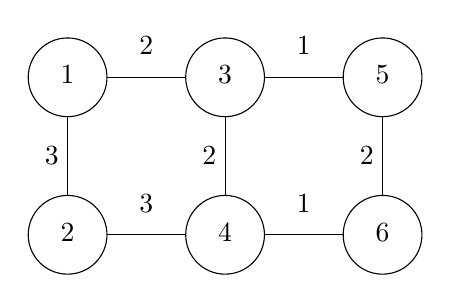
\begin{tikzpicture}
  %ノード1  
  \draw(4,2) circle (0.5)
  node[at={(4.0,2.0)}] {
    \begin{tabular}{c}
      1
    \end{tabular}
  };
  %ノード2  
  \draw(4,0) circle (0.5)
  node[at={(4.0,0.0)}] {
    \begin{tabular}{c}
      2
    \end{tabular}
  };
  %ノード3  
  \draw(6,2) circle (0.5)
  node[at={(6.0,2.0)}] {
    \begin{tabular}{c}
      3
    \end{tabular}
  };
  %ノード4  
  \draw(6,0) circle (0.5)
  node[at={(6.0,0.0)}] {
    \begin{tabular}{c}
      4
    \end{tabular}
  };
  %ノード5  
  \draw(8,2) circle (0.5)
  node[at={(8.0,2.0)}] {
    \begin{tabular}{c}
      5
    \end{tabular}
  };
  %ノード6  
  \draw(8,0) circle (0.5)
  node[at={(8.0,0.0)}] {
    \begin{tabular}{c}
      6
    \end{tabular}
  };
  \draw(4,0.5) --(4,1.5)
  node[at={(3.8,1.0)}] {3};
  \draw(6,0.5) --(6,1.5)
  node[at={(5.8,1.0)}] {2};
  \draw(8,0.5) --(8,1.5)
  node[at={(7.8,1.0)}] {2};
  \draw(4.5,0) --(5.5,0)
  node[at={(5.0,0.4)}] {3};
  \draw(4.5,2) --(5.5,2)
  node[at={(5.0,2.4)}] {2};
  \draw(6.5,0) --(7.5,0)
  node[at={(7.0,0.4)}] {1};
  \draw(6.5,2) --(7.5,2)
  node[at={(7.0,2.4)}] {1};
\end{tikzpicture}

\caption{重み付き無向グラフの例}
\label{graphexample}
\end{figure}
%%%%%%%%%%%%%%%%%%%%%%%%%%%%%%
\lstinputlisting[float=t,caption={%
グラフ(図~\ref{graphexample})のASPファクト表現},%
captionpos=b,frame=single,label=code:graph_example.lp,%
numbers=none,%
breaklines=true,%
columns=fullflexible,keepspaces=true,%
basicstyle=\ttfamily\scriptsize]{code/graph_example.lp}
%%%%%%%%%%%%%%%%%%%%%%%%%%%%%%

最短ハミルトン閉路問題を例にとって,
入力となる重み付き無向グラフ(図~\ref{graphexample})の
ASP ファクト形式をコード~\ref{code:graph_example.lp}に示す.
%
アトム\code{node/1}は頂点,\code{edge/2}は辺,\code{cost/3}は距離を表す.
例えば,
\code{edge(1,2)}は,辺
\code{1}~--~\code{2}を表し,
\code{cost(1,2,3)}は,この辺の重みが\code{3},
すなわち,頂点\code{1} と頂点\code{2}の距離が
\code{3}であることを示している.

%%%%%%%%%%%%%%%%%%%%%%%%%%%%%%%%%%%%%%%%%%%%%%%%%%%%%%%%%%%%%%%%%%%%%%%
\subsection{\textsf{undirected}符号化}
%%%%%%%%%%%%%%%%%%%%%%%%%%%%%%%%%%%%%%%%%%%%%%%%%%%%%%%%%%%%%%%%%%%%%%%

%%%%%%%%%%%%%%%%%%%%%%%%%%%%%%
\lstinputlisting[float=t,caption={%
\textsf{undirected}符号化},%
captionpos=b,frame=single,label=code:hamilton1.lp,%
numbers=left,%
breaklines=true,%
columns=fullflexible,keepspaces=true,%
basicstyle=\ttfamily\footnotesize]{code/hc_undirected.lp}
%%%%%%%%%%%%%%%%%%%%%%%%%%%%%%

グラフ$G=(V,E)$にハミルトン閉路が存在する必要十分条件は,
以下の2つの制約を満たす部分グラフ$G'=(V,E')$が存在することである.
\begin{itemize}
\item $G'$の各頂点の次数が2 (次数制約)
\item $G'$が連結である (連結制約)
\end{itemize}
ハミルトン路の場合,次数制約は
「始点と終点の次数が1,他の頂点の次数が2」となる.

\textsf{undirected}符号化は,ハミルトン閉路問題の次数制約と連結制約を,
ASP の一貫性制約と個数制約を使って表した基本的な符号化である.
コード~\ref{code:hamilton1.lp}に\textsf{undirected}符号化を示す.
コード中の\code{s}は始点の頂点番号を表し,実際の値は実行時に与えられる.
\begin{itemize}
\item 1行目のルールは,各辺\code{edge(X,Y)}に対して,その辺がハミルト
  ン閉路に含まれるかどうかを意味するアトム\code{in(X,Y)}を選択子を使っ
  て導入している.
\item 次数制約は3行目のルールで表される.
  このルールは,各頂点\code{node(X)}に対して,
  その次数が2に等しくなることを個数制約を使って表している.
\item 連結制約は4--7行目のルールで表される.
  ある頂点\code{X}が始点\code{s}から到達可能であることを意味する補助ア
  トム\code{reached(X)}を導入する.
  4行目のファクトは,始点\code{s}が到達可能あることを表している.
  5行目のルールは,各辺\code{X}~--~\code{Y}に対して,その辺がハミルト
  ン閉路に含まれ(\code{in(X,Y)}),かつ,頂点\code{X}が始点から到達可能
  であれば(\code{reached(X)}),\code{Y}も到達可能であることを表している.
  6行目は5行目と同様であるが,辺を逆向きに辿った場合を表している.
  7行目のルールは,すべての頂点が始点から到達可能でなければならないこ
  とを一貫性制約を使って表している.
\end{itemize}
このように,\textsf{undirected}符号化は,ハミルトン閉路問題の次数制約
と連結制約を,ASPのルール6個で簡潔に表現している.
特に,4--7行目のように連結制約を簡潔に記述できる点は,ASP の大きな特長
の一つである.

%%%%%%%%%%%%%%%%%%%%%%%%%%%%%%%%%%%%%%%%%%%%%%%%%%%%%%%%%%%%%%%%%%%%%%%
\subsection{\textsf{directed}符号化}
%%%%%%%%%%%%%%%%%%%%%%%%%%%%%%%%%%%%%%%%%%%%%%%%%%%%%%%%%%%%%%%%%%%%%%%

%%%%%%%%%%%%%%%%%%%%%%%%%%%%%%
\lstinputlisting[float=t,caption={%
\textsf{directed}符号化},%
captionpos=b,frame=single,label=code:hamilton2.lp,%
numbers=left,%
breaklines=true,%
columns=fullflexible,keepspaces=true,%
basicstyle=\ttfamily\footnotesize]{code/hc_directed.lp}
%%%%%%%%%%%%%%%%%%%%%%%%%%%%%%

\textsf{directed}符号化は,\textsf{undirected}符号化をベースに,
与えられた無向グラフの各辺$u-v$に対して,2つの弧$u\rightarrow v$と
$v\rightarrow u$を対応させることで有向グラフ化して解く符号化である.
コード~\ref{code:hamilton2.lp}に,\textsf{directed}符号化を示す.
\begin{itemize}
\item 1行目では,無向グラフの有向グラフ化を行う.
  与えられた無向グラフの各辺\code{edge(X,Y)}に対して,
  2つの弧\code{in(X,Y)}と\code{in(Y,X)}を導入し,
  それらの高々1個がハミルトン閉路に含まれることを個数制約を使って
  表している.
\item 次数制約は2--3行目のルールで表される.
  2行目のルールは,各頂点\code{node(X)}の出次数が1に等しいことを表して
  いる.同様に,3行目のルールは入次数が1に等しいことを表す.
\item 連結制約は,\textsf{directed}符号化と同様に,
  補助アトム\code{reached/1}を使って表される(5--7行目).
\item 有向グラフ化した場合,
  無向グラフ上の各ハミルトン閉路に対して,
  右回りと左回りの2つの対称なハミルトン閉路が存在する.
  9行目のルールは,この対称解を除去する制約である.
\end{itemize}

%%%%%%%%%%%%%%%%%%%%%%%%%%%%%%%%%%%%%%%%%%%%%%%%%%%%%%%%%%%%%%%%%%%%%%%
\subsubsection{\textsf{acyclicity}符号化}
%%%%%%%%%%%%%%%%%%%%%%%%%%%%%%%%%%%%%%%%%%%%%%%%%%%%%%%%%%%%%%%%%%%%%%%

%%%%%%%%%%%%%%%%%%%%%%%%%%%%%%
\lstinputlisting[float=t,caption={%
\textsf{acyclicity}符号化},%
captionpos=b,frame=single,label=code:hamilton3.lp,%
numbers=left,%
breaklines=true,%
columns=fullflexible,keepspaces=true,%
basicstyle=\ttfamily\footnotesize]{code/hc_acyclicity.lp}
%%%%%%%%%%%%%%%%%%%%%%%%%%%%%%

\textsf{acyclicity}符号化は,\textsf{directed}符号化をベースに,
連結制約を部分閉路を禁止する制約に置き換えたものである.
コード~\ref{code:hamilton3.lp}に,\textsf{acyclicity}符号化を示す.
\textsf{directed}符号化との違いは,5行目だけである.
\begin{itemize}
\item 5行目のルールは,始点\code{s}を含まない弧\code{in(X,Y)}
  の集合をもつ有向グラフが閉路を含まないことを,
  {\clingo}の\code{\#edge}宣言を使って簡潔に表している.
\end{itemize}

%%%%%%%%%%%%%%%%%%%%%%%%%%%%%%%%%%%%%%%%%%%%%%%%%%%%%%%%%%%%%%%%%%%%%%% 
\subsection{最短ハミルトン閉路問題}\label{minexpl}
%%%%%%%%%%%%%%%%%%%%%%%%%%%%%%%%%%%%%%%%%%%%%%%%%%%%%%%%%%%%%%%%%%%%%%% 

%%%%%%%%%%%%%%%%%%%%%%%%%%%%%%
\lstinputlisting[float=t,caption={%
目的関数},%
captionpos=b,frame=single,label=code:obj_minimize.lp,%
numbers=none,%
breaklines=true,%
columns=fullflexible,keepspaces=true,%
basicstyle=\ttfamily\footnotesize]{code/obj_minimize.lp}
%%%%%%%%%%%%%%%%%%%%%%%%%%%%%%
\lstinputlisting[float=t,caption={%
補助ルール},%
captionpos=b,frame=single,label=code:cost_both.lp,%
numbers=none,%
breaklines=true,%
columns=fullflexible,keepspaces=true,%
basicstyle=\ttfamily\footnotesize]{code/cost_both.lp}
%%%%%%%%%%%%%%%%%%%%%%%%%%%%%%


最短ハミルトン閉路問題のASP符号化は,これまで説明した各符号化に,
目的関数を追加することで実現できる.
\textsf{undirected}符号化の場合は,
コード~\ref{code:obj_minimize.lp}のルールを追加すればよい.
%
この\code{#minimize}宣言は,
ハミルトン閉路に含まれる各辺\code{X}~--~\code{Y}の距離\code{C}
の総和を最小化することを意味する.
%
\textsf{directed}と\textsf{acyclicity}符号化については,
無向グラフの各辺\code{edge(X,Y)}に対して,2つの弧\code{in(X,Y)}と
\code{in(Y,X)}を導入している.
そのため,上記の\code{#minimize}宣言に加えて,
コード~\ref{code:cost_both.lp}の補助ルールを追加する必要がある.

%%%%%%%%%%%%%%%%%%%%%%%%%%%%%%%%%%%%%%%%%%%%%%%%%%%%%%%%%%%%%%%%%%%%%%% 
\subsection{コスト制約付きハミルトン閉路問題}
%%%%%%%%%%%%%%%%%%%%%%%%%%%%%%%%%%%%%%%%%%%%%%%%%%%%%%%%%%%%%%%%%%%%%%% 

%%%%%%%%%%%%%%%%%%%%%%%%%%%%%%
\lstinputlisting[float=t,caption={%
コスト制約},%
captionpos=b,frame=single,label=code:cost_constraint.lp,%
numbers=none,%
breaklines=true,%
columns=fullflexible,keepspaces=true,%
basicstyle=\ttfamily\footnotesize]{code/cost_constraint.lp}
%%%%%%%%%%%%%%%%%%%%%%%%%%%%%%

コスト制約付きハミルトン閉路問題は,
ハミルトン閉路問題に,距離の総和が所与の閾値以下であるこ
とを制約条件として付加した問題である.
この問題のASP符号化は,
ハミルトン閉路問題の\textsf{undirected}, \textsf{acyclicity},
\textsf{directed}符号化に,
コード~\ref{code:cost_constraint.lp}のルールを追加することで実現できる.
%
コード中の\code{c}は閾値を表し,実際の値は実行時に与えられる.
また,最短ハミルトン閉路問題の場合と同じ理由で,
\textsf{directed}と\textsf{acyclicity}符号化については,
アトム\code{cost/3}に関する補助ルール(コード~\ref{code:cost_both.lp})
も追加する必要がある.

%%%%%%%%%%%%%%%%%%%%%%%%%%%%%%%%%%%%%%%%%%%%%%%%%%%%%%%%%%%%%%%%%%%%%%%
%%% Local Variables:
%%% mode: latex
%%% TeX-master: "paper"
%%% End:
